%%%%%%%%%%%%%%%%%%%%%%%%%%%%%%%%%%%%%%%%%%%%%%%%%%%%%%%%%%%%%%%%%%%%%%%%%%%%%%%%%%
% 1
%%%%%%%%%%%%%%%%%%%%%%%%%%%%%%%%%%%%%%%%%%%%%%%%%%%%%%%%%%%%%%%%%%%%%%%%%%%%%%%%%%

\section{Breast Cancer Detection}

\subsection{Medical imagery screening tests \& biopsies}
\label{sec:litreview-bcd-medical-imagery}

Test screenings have been used to detect early signs of breast cancer before the appearance of any symptoms, such as lumps that can be felt to the touch of a hand. The main methods used for breast cancer screenings are \textit{mammograms}, which are low-dosage x-rays around the breast area usually  used as initial/regular screening tests. This screening method is followed by \textit{breast ultrasounds} for analysing masses such as lumps or cysts, and by \textit{breasts MRI} (Magnetic Resonance Imaging) for detailed imagery of the breast, usually used to when a cancer has already been diagnosed to get more information about the tumour, such as its size and location, or to find additional ones \citep{americanCancerSociety2019}. If any of the aforementioned screening tests raise suspicion or reveal a potential presence of breast cancer, then biopsies can be conducted to confirm the screening tests' results. Biopsies consist of extracting cells or a small part of the breast's tissue that are sent to a lab to be analysed by pathologists to get definite results \citep{martin2019}.\\

Due to the invasive nature of biopsies, it is ideal for patients to use medical imagery tools to detect early signs of breast cancer that can be treated efficiently rather than immediately conducting a biopsy. Mammograms are the primary imagery method used for early breast cancer detection (BCD) \citep{Ramos-Pollan2012}. However, breast cancer detection using mammograms, and any form of cancer using medical imagery, relies on the conventional diagnoses of expert radiologists \citep{Osareh2010}. These diagnoses rest on the correct interpretation of the mammograms, which may be subject to errors due to the difficulty of correctly interpreting them \citep{Elter2009}. Indeed, mammograms are 2D images of 3D breasts that correspond to the superposition of breast tissue, which increases the difficulty for a radiologist to correctly analyse patterns as masses often naturally form due to this superposition \citep{Elter2009}.

\subsection{Early Breast Cancer Detection Systems}
\label{sec:litreview-bcd-early-cad}

% todo: explain what are mammograms -> support for why it's hard for radiologists alone to make decisions based on mammograms
% limitations of radiologists

To assist radiologists in their interpretations of mammograms, Computer-Assisted Detection/Diagnosis (CAD) software have been employed since the 1970s. However, pre-1990s CAD systems were very primitive and did not offer much more knowledge than the expert radiologists' knowledge. These unsophisticated ``expert'' systems consisted of manually processing and modelling pixels to construct rule-based systems that mainly used \textit{if-else-then} statements \citep{Litjens2017}, highlighting their inadequacy to learn how to recognise patterns that can be used to detect breast cancer.

\begin{figure}[ht]
\centerline{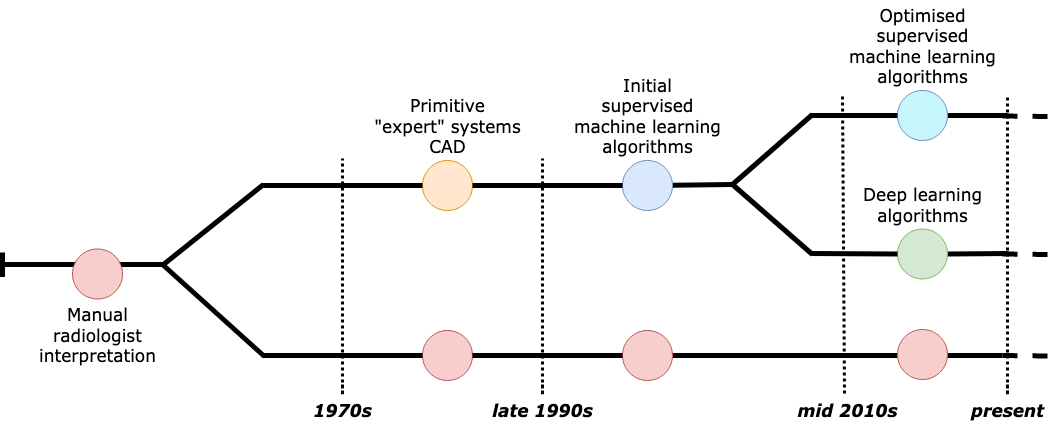
\includegraphics[width=\textwidth]{Dissertation/figures/litsurvey/bcd_timeline.png}}
\caption{\label{fig:litsurvey-bcd-timeline}Timeline of the evolution of breast cancer detection systems synthesising the information described in Sections~\ref{sec:litreview-bcd-medical-imagery}~and~\ref{sec:litreview-bcd-early-cad}. Created using draw.io.}
\end{figure}

\subsection{Towards Supervised Machine Learning-based Systems}

Towards the late 1990s, supervised machine learning techniques started replacing these expert systems, allowing hidden patterns in the mammograms' data that could not be perceived by radiologists to now be recognised by these new algorithms. Machine learning-based approaches were selected over statistical approaches as they were more performant when dealing with large, complex and high-dimensional datasets \citep{Yue2018}, which is the case of datasets of mammograms. Additionally, machine learning methods were proven to be more suitable for the task of classification than traditional statistics-based approaches such as regression \citep{Paliwal2009}. This marked the shift from CAD systems that were fully designed by humans to systems that were trained on datasets of medical imagery \citep{Litjens2017}.\\

However, these machine learning models could not accurately operate on purely raw data such as the full-sized mammogram images. Indeed, all of the machine learning models tested against the task of breast cancer detection required relevant pieces of information to first be extracted from the image to solve the given task, such as k-Nearest Neighbour [kNN], Decision Trees [DT], Naive Bayes [NB] \citep{Asri2016}, Support Vector Machines [SVM] \citep{Ramos-Pollan2012} and Artificial Neural Networks [ANN] \citep{Yue2018}. These important bits of information pulled from the mammograms data correspond to features, and need to be extracted by humans before being fed to the aforementioned models for training. These features range from visual information, such as colours, edges, corners, shapes and textures \citep{Geron2019}, to extracted information, such as the cell size, clump thickness, bare  nuclei, etc. \citep{Yue2018}.\\

Logically, the next step in the evolution of breast cancer detection systems is for the model to learn these features on its own directly from the data rather than being fed hand-extracted features \citep{Yala2019}. Deep learning models, which corresponds to neural networks with hundreds of hidden layers, are based on this concept and are covered in Section~\ref{sec:litsurvey-DLtechniques-CNN}. However, these models have not been successfully implemented until recent years as they require powerful computers, usually equipped with Graphical Processing Units (GPU) to be efficiently trained. This means that until recent years, the machine learning models discussed in Section~\ref{sec:litreview-MLmodel-BCDapplications} have led the field of breast cancer detection, with some manual mammogram interpretations still being carried out by radiologists \citep{Litjens2017}, as depicted in Figure~\ref{fig:litsurvey-bcd-timeline}.

% History of breast cancer detection (leads to)\\
% Motivation of using ML/DL for breast detection\\
% Problems with current breast cancer detection systems

%%%%%%%%%%%%%%%%%%%%%%%%%%%%%%%%%%%%%%%%%%%%%%%%%%%%%%%%%%%%%%%%%%%%%%%%%%%%%%%%%%
% 2
%%%%%%%%%%%%%%%%%%%%%%%%%%%%%%%%%%%%%%%%%%%%%%%%%%%%%%%%%%%%%%%%%%%%%%%%%%%%%%%%%%

\section{Machine Learning Tasks \& Algorithms}
\label{sec:litreview-MLmodel-BCDapplications}

\subsection{Machine Learning Applications to Breast Cancer Detection}

\subsubsection{Types of machine learning algorithms}

Machine learning algorithms fall in different categories based on whether human supervision is required or not. The two main types of machine learning algorithms correspond to supervised and unsupervised learning. On the one hand in supervised learning, the dataset is labelled, meaning every sample in the dataset includes a solution \citep{Geron2019}. This label, often noted $y$, is used to make a prediction $\hat{y}$ by fitting the input features $\textbf{x}$ from a training dataset. The goal of a supervised learning algorithm is to determine the optimal parameters $\theta$ for the selected algorithm in order to minimise a loss function defined as $L(y,\hat{y})$, which corresponds to the error between the predicted algorithm's output $\hat{y}$ and the real output $y$ \citep{Litjens2017}. A large variety of loss functions can be used such as the general Mean Squared Error (MSE) and Mean Absolute Error (MAE) loss functions, or more specific loss functions such as the Hinge Loss for SVMs \citep{Geron2019}. The main applications of supervised learning are classification and regression, with the former being the most relevant to breast cancer detection.\\

On the other hand in unsupervised learning, the data is unlabelled, meaning only the input features $\textbf{x}$ are available while the labels $y$ are not \citep{Litjens2017}. This means the algorithm cannot optimise its hyperparameters by minimising a loss function. Instead, the algorithm needs to automatically create clusters in the dataset in order to separate them into different groups. The main applications of unsupervised learning are clustering, anomaly detection, data visualisation and dimensionality reduction \citep{Geron2019}, rendering them irrelevant to the breast cancer detection. Two other categories of machine learning algorithms exist, corresponding to semi-supervised learning and reinforcement learning, but are also irrelevant to the task of detecting breast cancer.\\

Among the aforementioned types of machine learning algorithms, the most pertinent one for the task of breast cancer detection is supervised learning as datasets of mammograms need to contain properly labelled data for each sample, indicating the status of the mammogram i.e. no tumour, benign tumour, malignant tumour \citep{Shen2017}.

\subsubsection{Types of machine learning tasks}

Two types of machine learning tasks are very relevant to medical imagery analysis, including mammogram analysis for breast cancer detection: \textit{detection} (classification) and \textit{segmentation} \citep{Litjens2017}. 

\paragraph{Detection} corresponds to the classification of a medical image or exam, which is an interpretation that used to be fully carried out by a radiologist before the appearance of CAD systems (see Section~\ref{sec:litreview-bcd-early-cad}). The classification can be either binary or multi-class depending on the data used. With datasets like the ``Curated Breast Imaging Subset of DDSM'' \citep{Lee2017}, the classification is binary as mammograms can only be classified as either ``benign'' or ``malignant''. However, when using datasets like the ``Digital Database for Screening Mammography'' \citep{DDSMdataset2001}, the classification becomes more interesting from a clinical point of  view as mammograms can either be classified as ``normal'', ``benign'' or ``malignant'' \citep{Litjens2017}. An example of a classification between benign and malignant mammograms can be found in Figure~\ref{fig:classification_example}, reinforcing the complexity that comes with interpreting mammograms for radiologists and the need for accurate and reliable CAD systems to improve the prediction accuracies.

\begin{figure}[h]
\centering
\begin{subfigure}{.5\textwidth}
  \centering
  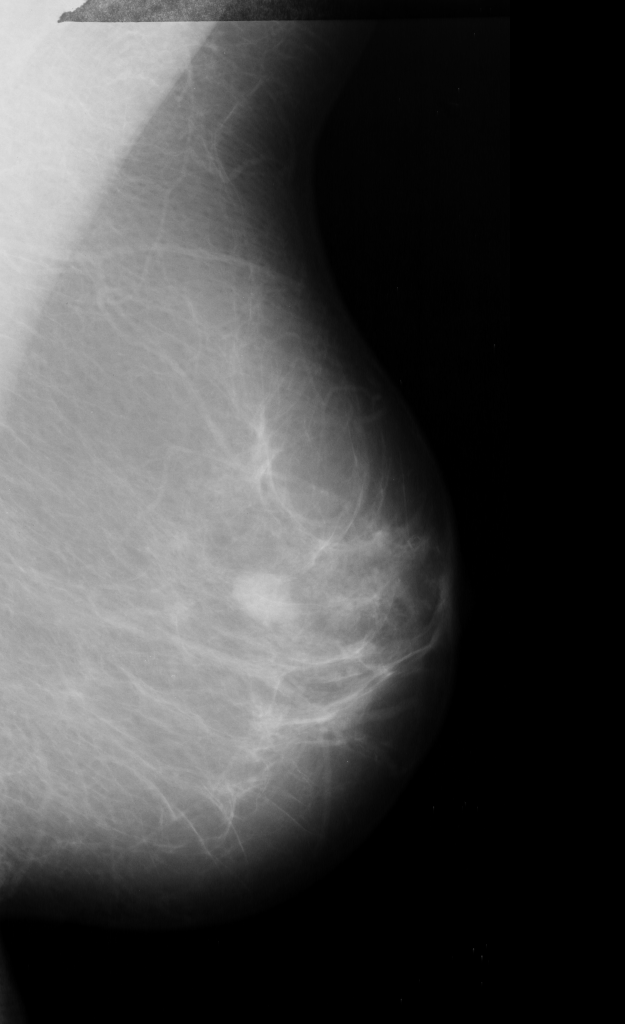
\includegraphics[width=0.5\textwidth]{Dissertation/figures/litsurvey/classification_benign.png}
  \caption{A benign mammogram.}
  \label{fig:classification_benign}
\end{subfigure}%
\begin{subfigure}{.5\textwidth}
  \centering
  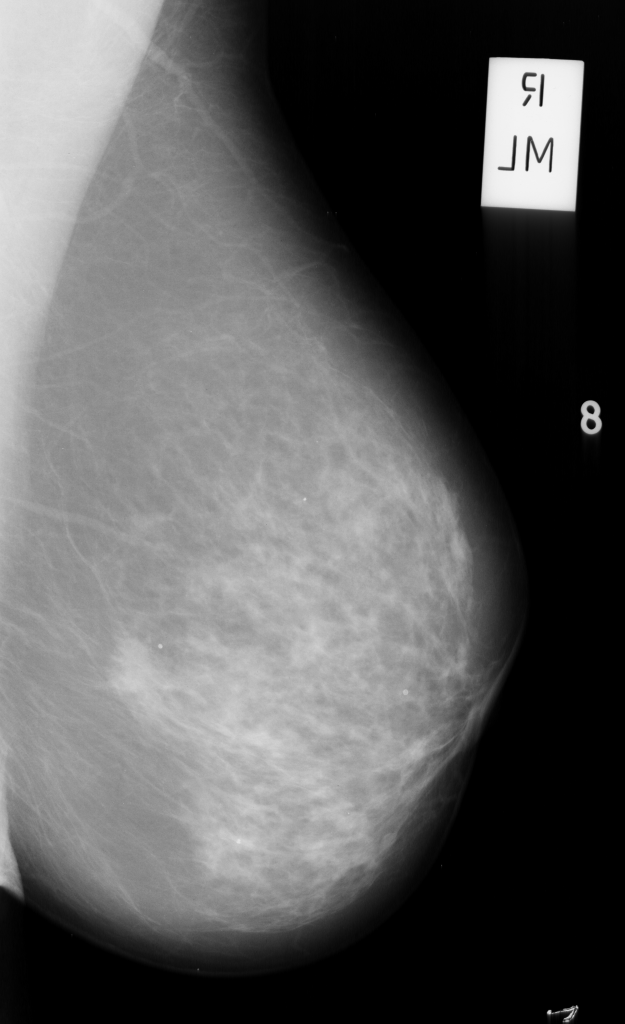
\includegraphics[width=0.5\textwidth]{Dissertation/figures/litsurvey/classification_malignant.png}
  \caption{A malignant mammogram.}
  \label{fig:classification_malignant}
\end{subfigure}
\caption{\label{fig:classification_example}Example of a breast mammogram classification, showing benign (left) and malignant (right) mammograms. Images retrieved from the mini-MIAS dataset (Suckling, 1994).}
\end{figure}

\paragraph{Segmentation} corresponds to the classification of each pixel in the image based on the class of the object the pixels belongs to, without distinguishing objects from the same class. All objects belonging to the same class will be classified in the same grouping of pixels \citep{Geron2019}. In breast cancer detection, segmentation can be used to highlight masses such as calcifications, cysts or fibroadenomas \citep{breastcancerorg2018} in mammograms by separating the masses from the background. An example is shown in Figure~\ref{fig:segmentation_example}, where mammograms are partitioned into non-overlapping segments, revealing potential masses in the image \citep{Punitha2018}.\\

\begin{figure}[h]
\centering
\begin{subfigure}{.5\textwidth}
  \centering
  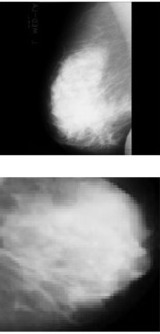
\includegraphics[width=0.52\textwidth]{Dissertation/figures/litsurvey/segmentation_example_original.jpg}
  \caption{Original mammogram images.}
  \label{fig:original-mammogram}
\end{subfigure}%
\begin{subfigure}{.5\textwidth}
  \centering
  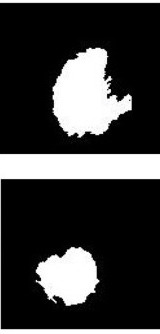
\includegraphics[width=0.52\textwidth]{Dissertation/figures/litsurvey/segmentation_example_segmented.jpg}
  \caption{Segmented mammogram images.}
  \label{fig:segmented-mammogram}
\end{subfigure}
\caption{\label{fig:segmentation_example}Example of a breast mammogram segmentation, showing the original mammogram (left) and the segmented image (right), depicting large masses. Images retrieved from Punithaet al. (2018).}
\end{figure}

Other machine learning tasks that have been used in medical imagery analysis consist of content-based image retrieval (retrieving similar images from a database) or image enhancement (erasing obstructing elements from an image and increasing quality) \citep{Litjens2017}, but will not be further explored as they are not directly relevant to the task of breast cancer detection. Indeed, the task of classification (detection) can be used to interpret whether a breast is affected by cancer through the analysis of databases of mammograms, while the task of segmentation can be used to localise a tumour within a breast by finding regions that may correspond to masses, pinpointing potential danger areas that may lead to cancerous cells.

\subsection{Comparison of BCD Supervised Learning Algorithms}

Since the late 1990s, a rich array of supervised machine learning algorithms have been applied and tested against the task of breast cancer detection, yielding varying results, but ultimately contributing to improving accuracies for detecting breast cancer \citep{Yue2018}. The main types of algorithms used in breast cancer detection, which consist of k-Nearest Neighbour (kNN), Naive Bayes (NB), Support Vector Machines (SVM), Decision Trees (DT) and Artificial Neural Networks (ANN), are briefly explained in the ensuing sections from most simple to most complex. Their performances when applied to the task of breast cancer detection are then compared to draw a picture of the advantages and disadvantages that each method brings.

\subsubsection{k-Nearest Neighbours}
\label{sec:litreview-knn}

k-Nearest Neighbours (kNN) is one of the simplest machine learning algorithms and is often used as an initial benchmark when studying a dataset with no prior knowledge \citep{peterson2009k}. It is a non-parametric and lazy model, as it does not learn the data's pattern but rather classifies a test sample by looking at its $k$ nearest neighbours \citep{Yue2018}. The sample data point's nearest neighbours are determined by using distance metrics such as the Euclidian distance, defined by Equation~\ref{eq:euclidian-distance} ($n$-dimensional space between two data points $s$ and $p$) which is the most widely used metric \citep{peterson2009k}. Figure~\ref{fig:litsurvey-knn-example} depicts an example of how a kNN classifier would be used to distinguish between a benign and a malignant tumour using $k=3$.

\begin{equation}
\label{eq:euclidian-distance}
    d(s,p)=\sqrt{\sum_{i=1}^{n}(s_i-p_i)^2}
\end{equation}

\begin{figure}[h]
\centerline{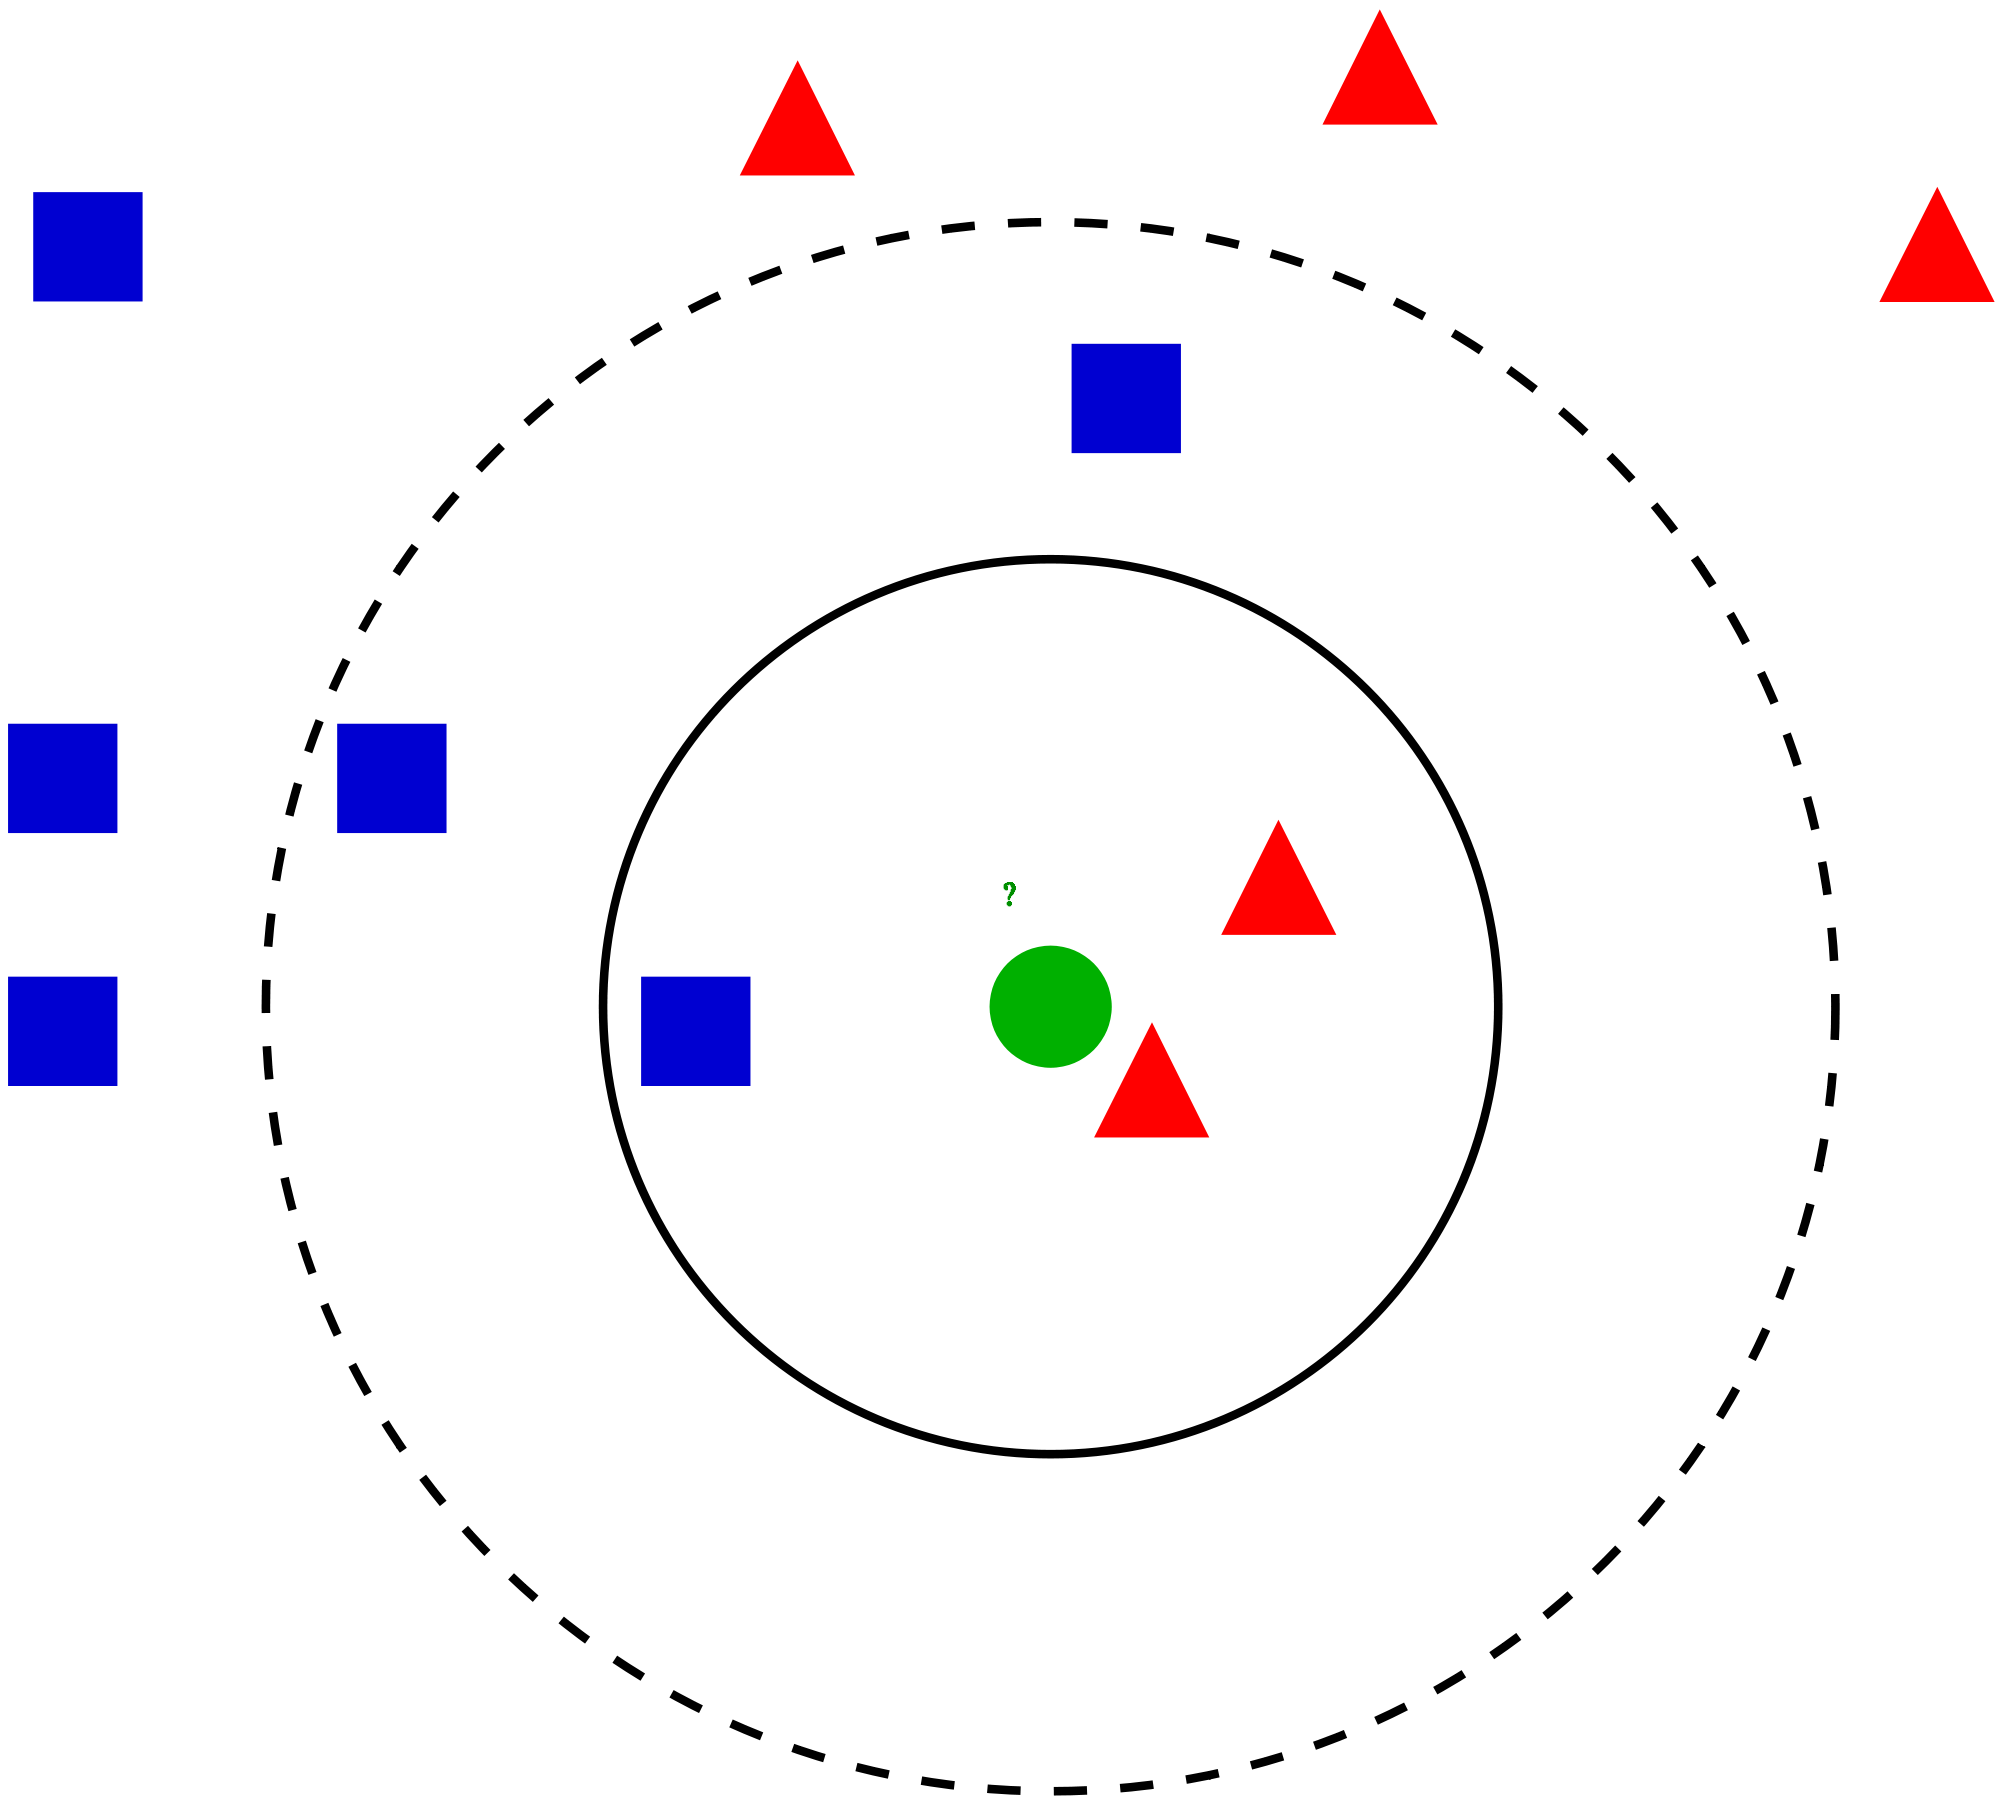
\includegraphics[width=0.4\textwidth]{Dissertation/figures/litsurvey/knn.png}}
\caption{\label{fig:litsurvey-knn-example}Example of a kNN classifier distinguishing between benign (blue square) and malignant (red triangle) tumours for a test data sample (green circle) using $k=3$. The test sample is classified as malignant as there are two red triangles and one blue square amongst the three neighbours. Figure retrieved online from T. Srivastava (\url{https://tinyurl.com/y3jqco49}).}
\end{figure}

Generally used as an initial learning algorithm to experiment with new datasets, the kNN algorithm has been tested on distinctive datasets of mammograms for breast cancer detection such the ``Wisconsin Breast Cancer Wisconsin'' (WBCD) dataset \citep{Wolberg1995}, which contains 10 extracted features such as clump thickness, cell size/shape, etc. \citep{Wolberg1995}. kNNs calibrated with $k=1$ and using the Euclidian distrance achieved 98.25\% accuracy \citep{Sarkar2000} and 98.70\% accuracy \citep{AhmedMedjahed2013} on the WBCD dataset when compared with other values of $k$ ranging from 1 to 15 and using other distance metrics such Cityblock distance, cosine distance and correlation.\\

Despite Sarkar et al. and Medjahed et al. reporting that a value of $k=1$ seemed to yield the most accuracy, these 1-NN classifiers do not actually learn the data's patterns and often underperform compared to other classifiers mentioned below, especially compared to SVMs and ANNs which can surpass accuracies of 99\% \citep{Yue2018, Asri2016, Montazeri2016}. Nevertheless, the results achieved by kNN remain fruitful when used as a basic benchmark before testing more advanced models, such as the ones described below.

\subsubsection{Naive Bayes}

Naive Bayes uses Bayes' theorem and the assumption that all input features are independent from one another, which can be described as the input features $\textbf{x}=(\textbf{x}_1, ..., \textbf{x}_n)$ being independent given a class label $C$ in Equation~\ref{eq:naive-bayes} \citep{rish2001empirical}.

\begin{equation}
\label{eq:naive-bayes}
    P(\textbf{x}|C)=\prod_{i=1}^{n}P(\textbf{x}_i|C)
\end{equation}

This assumption leads to a naive model that despite not learning the data's underlying pattern (in a similar fashion to kNN), still offers competitive results in practice \citep{russell2002artificial}, notably in the field of medical imagery analysis \citep{rish2001empirical}. Naive Bayes achieves an accuracy of 93\% on the WBCD dataset \citep{Kharya2014}, which is comparable to the aforementioned 1-NN classifiers as it does not learn the data's patterns and use extracted features rather than the original mammograms. NB still remains useful for assessing benchmark classification to compare with more advanced models.

\subsubsection{Decision Trees}

Unlike kNN and NB, the decision tree algorithm is a simple yet powerful one that fits the data. It works like a flowchart mapping samples' input feature vectors attributes and values, creating a tree made up of different types of nodes. Each non-leaf nodes tests one of the feature vectors attributes, branching out to a deeper node based on the attribute's value. Once a leaf node is reached after multiple tests, a classification decision is made \citep{quinlan2014c4}. An example of a decision tree applied to breast cancer detection can be found in Figure~\ref{fig:litsurvey-dt-example}, illustrating how attributes and their values are used to classify a tumour as benign or malignant.\\

\begin{figure}[ht]
\centerline{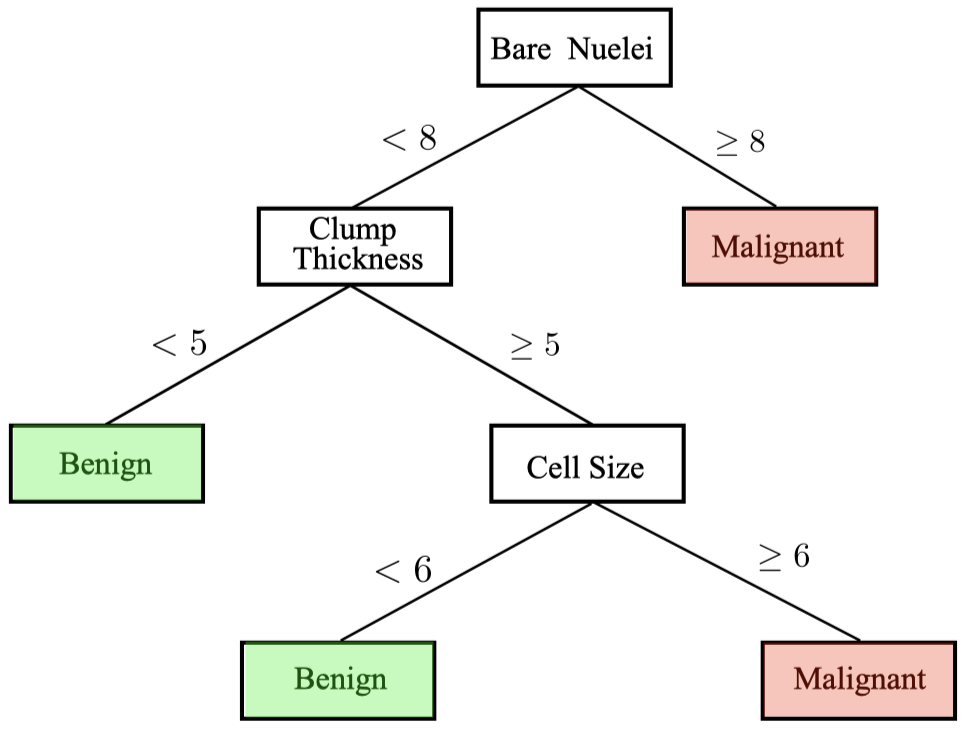
\includegraphics[width=0.65\textwidth]{Dissertation/figures/litsurvey/dt.png}}
\caption{\label{fig:litsurvey-dt-example}Example of a decision tree classifier distinguishing between benign and malignant tumours based on three extracted features from a dataset of mammograms: the size of the bare nuclei, the thickness of the clump and the uniformity of the cell size. Figure created by Yue et al. (2018).}
\end{figure}

The most popular implementations of decision trees use entropy-based impurity metrics to generate the tree, such as the ID3, C4.5 and C5.0 decision tree algorithms \citep{Yue2018}. A node reaches an entropy value of 0 when it is ``pure'' i.e. it contains only instances of one class (either only benign or only malignant data samples) \citep{Geron2019}.\\

The extra complexity offered by decision trees such as the C4.5 classifier does do not offer improved results compared to kNN and NB classifiers, with 94.56\% achieved using J48 (Java implementation of C4.5) on the WBCD dataset \citep{Sumbaly2014}, which is still falling short of the performance achieved by SVMs and ANNs, which can exceed the 99\% threshold \citep{Yue2018}. Nevertheless, inserting decision trees into hybrid systems by combining them with other machine learning algorithms such as SVMs and NBs increases the accuracy to 97.13\% on the WBCD dataset \citep{Kumar2017}, which are closer to thos achieved by SVMs and ANNs \citep{Yue2018}. Indeed, these hybrid systems use the advantages of each method, cancelling out the negatives of each, but come at the cost of being complicated to engineer and still requiring handcrafted features to be fed to them as input, which is confirmed by the choice of testing these algorithms on the WBCD dataset rather than datasets containing raw images like DDSM.

\subsubsection{Support Vector Machines}

An SVM consist of a \textit{maximal margin classifier}, which aims to find the hyperplane that separates two classes the most, and the \textit{kernel trick}, used to separate non-linear data. In Figure~\ref{fig:litsurvey-svm-example}, a visual example of a maximum margin hyperplane to separate linearly separable benign and malignant tumours is shown. In the case of non-linear data, the training data is mapped to a higher dimension where they can be linearly separated. This is achieved by using the kernel trick, which maps the input feature vector to a higher dimension by using the dot product, but does not carry out the transformation, which would exponentially increase the size of the feature space and consequently the training time \citep{Geron2019}. This kernel trick is what allowed SVMs to become one of the most widely used machine learning models nowadays in many fields including medical imagery analysis \citep{Yue2018}.\\

\begin{figure}[ht]
\centerline{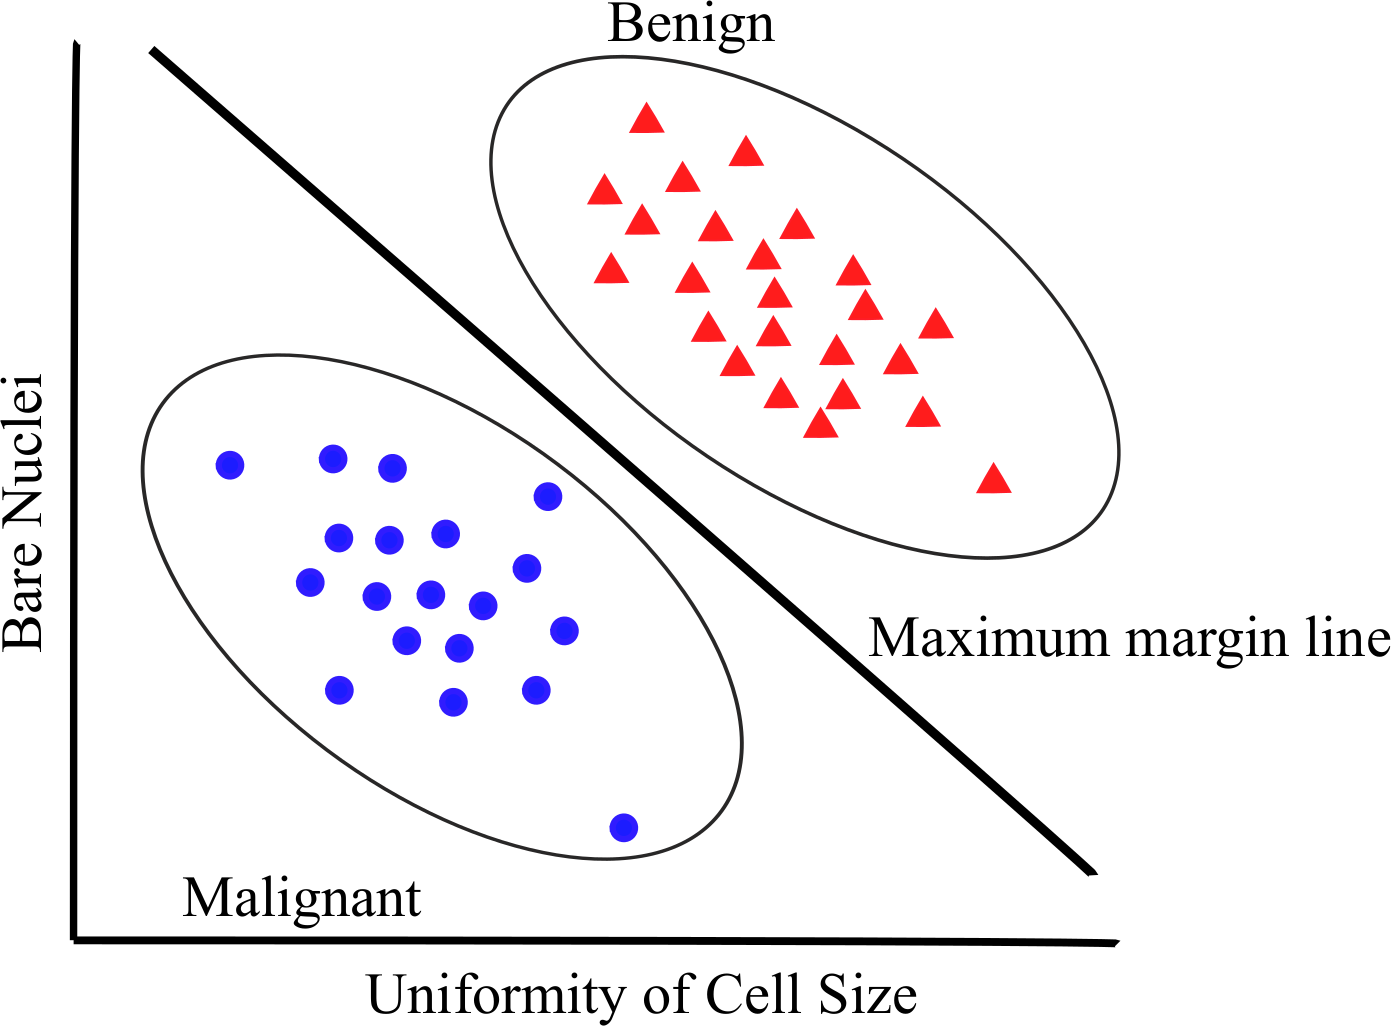
\includegraphics[width=0.6\textwidth]{Dissertation/figures/litsurvey/svm.png}}
\caption{\label{fig:litsurvey-svm-example}Example of a SVM classifier's maximum margin hyperplane found to separate benign and malignant tumours based on two extracted features from a dataset of mammograms: the size of the bare nuclei and the uniformity of the cell size. Figure created by Yue et al. (2018).}
\end{figure}

Many kernels can be chosen for SVM classification ranging from Polynomial kernel for image processing to Radial Basis Function (RBF) or Gaussian kernels for general tasks when there is no prior knowledge of the data), heavily influencing its performance \citep{amari1999improving}. For the task of breast cancer detection, RBF outperformed Polynomial kernels on two small datasets\footnote{``Fine needle aspirate of breast lesions'' (FNAB) dataset and ``gene microarrays'' dataset \citep{Osareh2010}.} containing extracted features, with the RBF kernel managing 98.80\% and 96.33\% accuracies on both datasets while Polynomial reached 97.09\% and 95\% accuracies \citep{Osareh2010}, depicting why RBF is often is often chosen over other kernels.\\

Compared to the previously mentioned ML methods, SVMs seem to learn the extracted features more efficiently, reaching 97.13\% accuracy on the WBCD, while kNN attained 95.27\%, NB 95.99\% and DT 95.13\% \citep{Asri2016}. When applied to datasets containing raw images such as CBIS-DDSM, SVMs coupled with feature extraction techniques such as gray-level co-occurence matrices (GLCM) achieved 63.03\% accuracy \citep{Sarosa2018}; while on smaller datasets like  mini-MIAS, SVMs coupled with texture-based features extracted from pre-processed images resulted in 92\% accuracy \citep{Vishrutha2014}. An accuracy of 97.2\% was achieved using the simplest form of SVMs on the WBCD dataset \citep{Bennett1998}, while 99.51\% accuracy was reached with SVMs on the same dataset when selecting the five best features \citep{Akay2009}, clearly characterising the importance of feature selection and image processing techniques for ML algorithms such as SVMs.

\subsubsection{Artificial Neural Networks}
\label{sec:litsurvey-anns}

ANNs form the basis of contemporary deep learning and are at the heart of the techniques mentioned in Section~\ref{sec:litsurvey-DLtechniques-CNN}. Originally inspired by the neuron connections found in the human brain \citep{mcculloch1943logical}, ANNs correspond to a collection of neurons (units) that ``fire'' an output if the linear sum of its weighted inputs tops a threshold. These neurons are placed in hierarchical layers (input, hidden and output layers) which are connected via weighted links, leading to \textit{fully connected} neural network when all the neurons from one layer communicate with all the neurons in the following layer. Input layer neurons accept the feature vectors $\textbf{x}$, hidden layer neurons process the data and output layer neurons represent an outcome for the classification \citep{russell2002artificial}. Figure~\ref{fig:litsurvey-ann-example} depicts an example fully-connected ANN used to classify benign and malignant tumours using six input neurons, eight hidden neurons and one output neuron.\\

\begin{figure}[ht]
\centerline{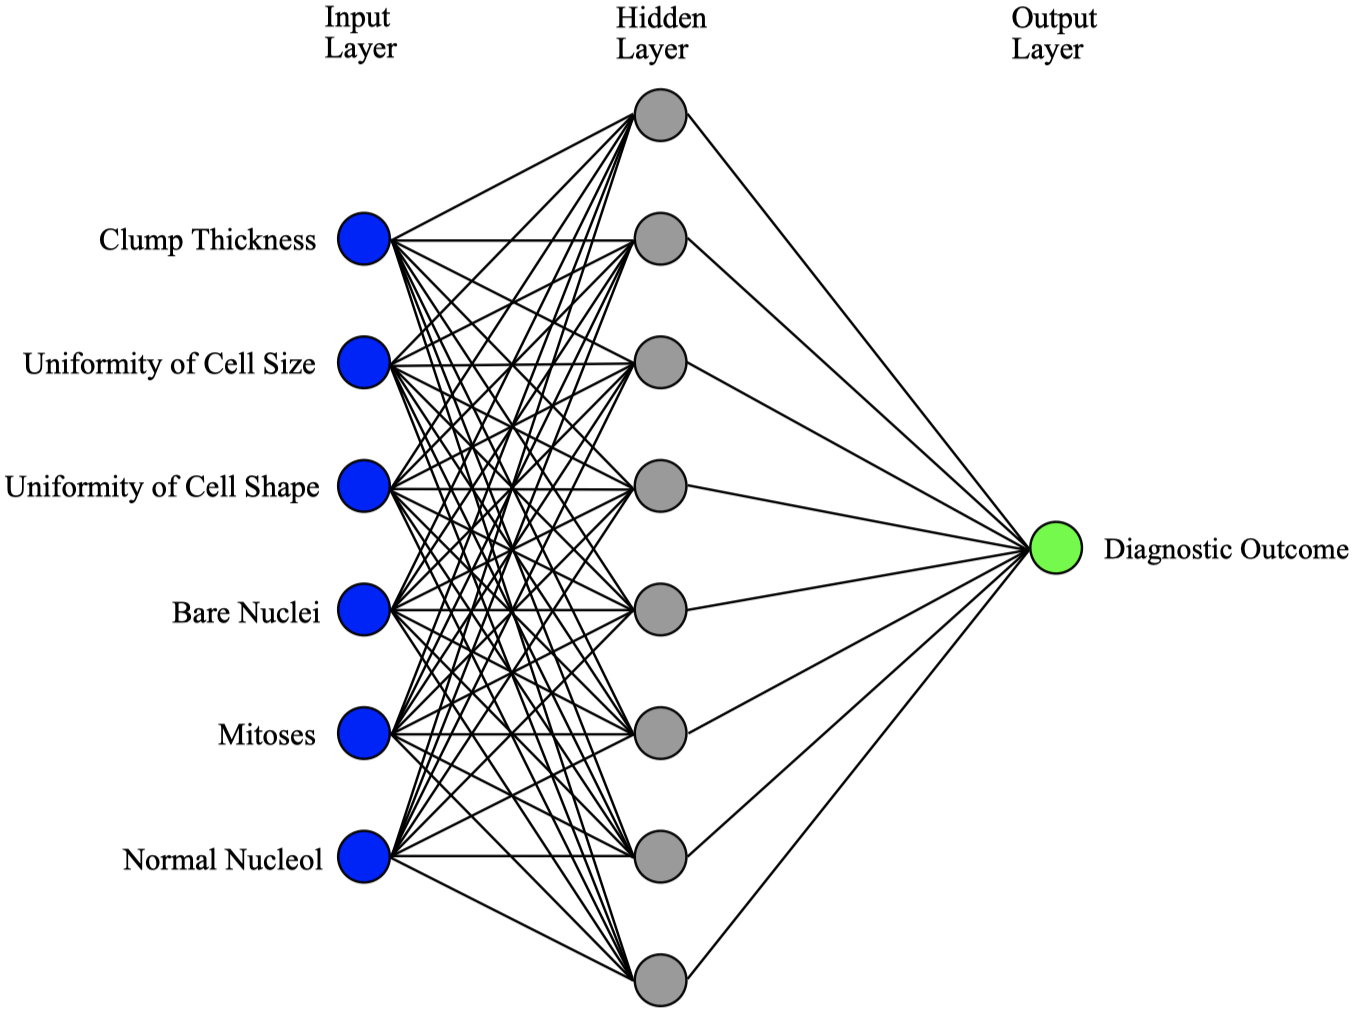
\includegraphics[width=\textwidth]{Dissertation/figures/litsurvey/ann.png}}
\caption{\label{fig:litsurvey-ann-example}Example of an ANN classifier distinguishing between benign and malignant tumours based on eight extracted features from a dataset of mammograms. Figure created by Yue et al. (2018).}
\end{figure}

Like the previous algorithms, neural networks learn by minimising the loss $L$ between the prediction $\hat{y}$ and the labels $y$. This is done via the backpropagation algorithm (BP), which backpropagates the error from the output layer to the hidden layers, allowing the links' weights to be adjusted to minimise that error \citep{russell2002artificial}. The most common way to do this is by using MLE with Stochastic Gradient Descent (SGD) \citep{Litjens2017}. This learning ability found in ANNs is what gives them their potential, but also their complexity due to the large number of hyperparameters used to fine-tune them and their capacity to overfit the data when over-engineered. Indeed, combinations of neural networks hyperparameters may involve the network's structure (number of layers and neurons in each layer), the learning rate and momentum, the regularisation parameters, the activation functions and the stopping conditions to name a few \citep{sklearn-MLP-2019}.\\
 
Shallow ANNs, also referred to as Multi-Layer Perceptrons, immediately showed promising results when first applied to breast cancer detection reaching 95\% accuracy \citep{Wu1993}. However, due to computational constraints, deeper ANNs containing multiple hidden layers could not be efficiently utilised until recent years \citep{Litjens2017}. Instead, innovative ANN variants have been used across the years to reduce training times, deal with multi-class classification with more ease, and yield more accurate classifications results comparable to the latest results achieved with SVMs. Some of these ANN variants include networks such as Probabilistic Neural Networks (PNN) that replace the classical sigmoid activation function with an exponential function to find the training sample that is closest to the testing sample \citep{Osareh2010}; or Genetically Optimised ANNs that use genetic programming (ML technique that evolves towards a solution based on Darwin's theory of evolution) to determine the best features to extract to optimise the networks weights and structure \citep{Bhardwaj2015}. These ANN variations reached 97.23\% and 99.26\% overall accuracies respectively.

% \begin{itemize}
%     \item Multi-Layer Perceptrons (shallow artificial neural networks)
%     \item Deep neural networks, problem with fully connected MLPs
% \end{itemize}

% \textit{For each, mention pros and cons based on existing papers and compare different approaches. Naturally lead towards deep neural networks (e.g. CNNs) for the final section.}

\subsubsection{Machine learning algorithms comparison}

The five previously explored supervised machine learning algorithms all have one commonality: they heavily rely on the quality of the features extracted from the mammogram images as input to gain performance rather than using the raw mammogram image as input. Additionally, the aforementioned algorithms all used the datasets containing extracted features such as the WBCD and XXX datasets, which only contain information extracted features from mammograms rather than actual mammogram imagery, reinforcing their incapability to learn directly from unprocessed \citep{Wolberg1995}.\\

On their own, each algorithm's limitations prevent it from performing well on large datasets. Combined to form hybrid systems, their accuracy is increased, but so is their complexity to setup correctly to avoid overfitting the data. Additionally, it is worth noting that considerable differences are achieved despite using identical algorithms due to diverse training strategies involving training/testing splits, the number of folds in cross-validation, the dataset used and the data pre-processing steps conducted \citep{Yue2018}.\\

The next step towards the evolution of these supervised learning algorithms is to redirect effort towards optimising and fine-tuning the hyperparameters and training strategies for these algorithms rather than extracting features to feed to these algorithms. The most efficient way nowadays to do so is through Convolutional Neural Networks (CNN), which ingest the raw mammogram images to learn which features to extract on their own and use them to detect instances of breast cancer.

% \begin{table}[h]
\centering
\resizebox{\textwidth}{!}{%
\begin{tabular}{l|l|l|l|l|l|}
\cline{2-6}
 &
  \textbf{kNN} &
  \textbf{NB} &
  \textbf{DT} &
  \textbf{SVM} &
  \textbf{ANN} \\ \hline
\multicolumn{1}{|l|}{\textbf{General Applications}} &
  N/A &
  N/A &
  N/A &
  N/A &
  N/A \\ \hline
\multicolumn{1}{|l|}{\textbf{Breast Cancer Detection Application}} &
  Basic benchmark &
  Basic benchmark &
  \begin{tabular}[c]{@{}l@{}}Low accuracies on its own.\\ High accuracies in hybrid systems.\end{tabular} &
   &
   \\ \hline
\end{tabular}%
}
\caption{Comparison of ML methods regarding general and BCD applications.}
\label{tab:my-table}
\end{table}

%%%%%%%%%%%%%%%%%%%%%%%%%%%%%%%%%%%%%%%%%%%%%%%%%%%%%%%%%%%%%%%%%%%%%%%%%%%%%%%%%%
% 3
%%%%%%%%%%%%%%%%%%%%%%%%%%%%%%%%%%%%%%%%%%%%%%%%%%%%%%%%%%%%%%%%%%%%%%%%%%%%%%%%%%

\section{Deep Learning techniques \& CNNs}
\label{sec:litsurvey-DLtechniques-CNN}

\subsection{Convolution Neural Networks}

\subsubsection{Motivation for CNNs over traditional neural networks}

CNNs are a type of neural network inspired by the human visual cortex, where neurons have local receptive fields that only react to visual stimuli originating from a region of the visual field. The combination of all receptive fields covered by overlapping neurons form the whole visual field \citep{Geron2019}. This architecture makes them very efficient at performing complex visual tasks, marked by the first milestone for CNNs with the LeNet-5 architecture trained to recognise handwritten bank cheque digits \citep{LeCun1998}.\\

CNNs differ from traditional ``shallow'' ANNs as they are not fully connected. Indeed, CNNs are partially connected, with neurons in one layer only connected to a few neurons from the previous layer, meaning that they can work with large images \citep{Geron2019}. In a fully-connected neural network with only 100 neurons in the first layer, a 1,000 x 1,000-pixel image would already have 100,000,000 connections\footnote{$1000 \cdot 1,000 = 1,000,000$ px; $1,000,000$px $\cdot 100$ neurons $= 100,000,000$ connections.} in that first layer alone. CNNs nowadays can work with images thousands of pixel large, including the ones found in mammogram datasets described in Chapter~\ref{ch:chapter-ethics-datasets}, processing them much faster than traditional machine learning methods.

\subsubsection{CNN Structure}

The structure of CNNs builds on top of the concepts of traditional ANNs (see Section~\ref{sec:litsurvey-anns}) by piling stack of convolutional layers and pooling layers that are followed by a fully connected network for classification (see Figure~\ref{fig:litsurvey-CNN-example}). The goal of the convolutional and pooling layers is to reduce the input images into a form that simple enough to be processed by other algorithms (the fully connected layers), retaining only useful information from the original image \citep{Shen2017}.

\begin{figure}[ht]
\centerline{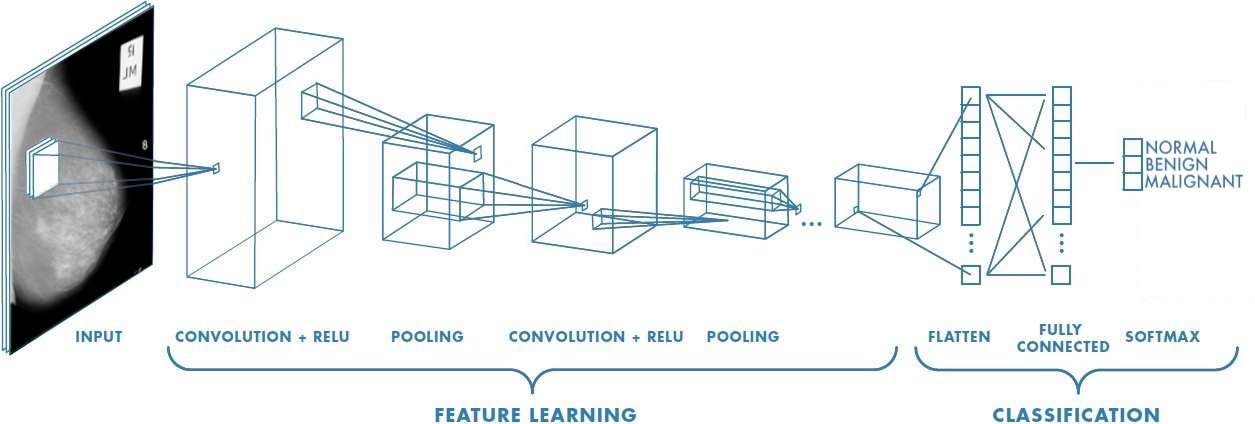
\includegraphics[width=\textwidth]{Dissertation/figures/litsurvey/CNN example.png}}
\caption{\label{fig:litsurvey-CNN-example}Example of a typical CNN adapted for multi-class breast cancer detection. Figure retrieved from S. Saha (\url{https://tinyurl.com/y9mmosuq}) and amended in Photoshop.}
\end{figure}

\paragraph{Convolution Layers \& Feature Maps}

Neurons in the first convolutional layers are only connected to pixels in their receptive fields and not connected to every pixel in the image. Similarly, neurons in deeper convolutional layers are only connected to neurons in a small zone from the previous layer. This allows the CNN to first focus on low-level features, which are progressively assembled into high-level features as the CNN gets deeper. The more the receptive fields are spaced out (defined as the stride), the smaller the next layer will be, thus considerably reducing the complexity of the CNN \citep{Geron2019}. Convolution is the mathematical operation that slides a moving a filter $f$ over an image $I$ to calculate a weighted sum (see Equation~\ref{eq:2d-convolution}). This 2D operation is possible in CNNs as layers are represented in 2D space and do not need to be flattened into a 1D array like with traditional neural networks, thus preserving the spatial information of images \citep{szeliski2010computer}.

\begin{equation}
\label{eq:2d-convolution}
    \hat{I}(x,y)=(I*f)(x,y)=\sum_{k}\sum_{l}I(k,l)\cdot f(x-k, y-l)
\end{equation}

The weights of the neurons in a convolutional layers correspond to the filters, which are learned during the training phase by using optimisation techniques such as gradient descent. These filters allow a layer of neurons to highlight the image areas that activate the filter the most. As each layer has multiple filters, different features can be simultaneously detected in the layer's input.\\

feature maps

\paragraph{Pooling Layers}

Pooling layers are similar to convolutional layers as neurons are only connected to neurons from a small region in the previous layer. The difference is that this layer is not trainable as its neurons have no weights. Indeed, it is only used to downsample the image as it traverses the network in order to diminish the load on the GPU. It does so by calculating an aggregate of its inputs based on a function, which can either be a maximum or an average function (see Figure~\ref{fig:litsurvey-max-vs-avg-pooling}). \textit{Maximum pooling} returns the maximum value of the covered portion of the image, whereas \textit{average pooling} returns the average of all values. Maximum pooling is the preferred option in CNNs as it retains the strongest features only and acts as a noise suppressant by discarding noisy activations \citep{Geron2019}.\\

\begin{figure}[ht]
\centerline{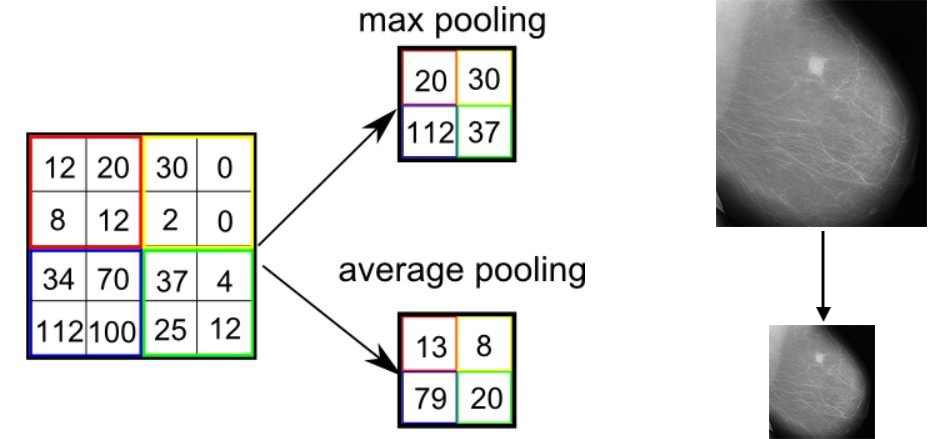
\includegraphics[width=\textwidth]{Dissertation/figures/litsurvey/max-vs-avg-pooling.png}}
\caption{\label{fig:litsurvey-max-vs-avg-pooling}Difference between max pooling and average pooling (left) to downsample an image (right). Figure retrieved from W. Ong (\url{https://tinyurl.com/y25cke6l}) and amended in Photoshop.}
\end{figure}

Other benefits of pooling layers are the lower memory usage and the number of trainable parameters linked to smaller images, and especially the invariance it provides to the CNN as it will not break down when fed images that contain features of different sizes than the ones seen in the training dataset \citep{Shen2017}.

\paragraph{Fully connected layers \& Activation functions}

Similarly to ANNs, activation functions are used to connect the convolutional and spooling layers. The most common activation function used in CNNs is the Rectified Linear Unit (ReLU).\\

At the end of the stack of convolutional and spooling layers, a fully connected MLP is placed. This dense neural network takes the flattened output of the convolutional and spooling layers (transformed from 2D to 1D), and performs the traditional classification tasks it was designed for using the features learned by the convolutional layers in a condensed  format. Depending on the number of classes to predict, a softmax activation can be used for multi-class classification or a sigmoid for binary classification.

\subsection{Applications to Breast Cancer Detection}

\subsubsection{CNN Architectures}

Applying VGG and ResNet CNN models to the task of breast cancer detection on the CBIS-DDSM

Evolution of CNNs (first CNN used, first CNN applied to medical imagery analysis, famous architectures e.g. LeNet-5, AlexNet, GoogLeNet, VGGNet, ResNet, Xception, SENet

% \begin{itemize}
%     \item Deep Neural Networks
%     \item Convolutional Neural Networks (losing resolution for segmentation due to downsampling layers)
% \end{itemize}

% Explore the techniques used in deep learning (techniques, databases, processing, libraries, output metrics, etc.)\\
% Explore the deep learning model that will be explored by each dissertation

\subsubsection{Rise of Deep Learning in Medical Imagery Analysis}

\paragraph{Main Challenges}

Implementing deep learning models requires a lot of data to achieve acceptable performance levels. However, labelled datasets are not always abundantly available as it requires a lot of time and resources to engineer large datasets with millions of images \citep{Krizhevsky2012} like ImageNet, which contains over 15 million high definition images from 15,000 different classes \citep{Deng2010}. With databases of mammograms barely exceeding 10,000 images, one of the challenges in implementing a deep learning CAD system is to overcome the small amount of data while avoiding overfitting it.

\paragraph{Transfer Learning}

A commonly used deep learning technique when only a little amount of data is available is transfer learning, which makes use of CNN models pre-trained on large general datasets. The knowledge gathered by high-performing CNNs in other general domains that have larger datasets can be transferred to a related domain such as medical imagery \citep{Falconi2019}.\\

These models are designed to classify millions of images across thousands of different classes and can easily be adapted to any classification task by replacing the dense output layer that makes the actual prediction with a layer containing one neuron per class to predict. In the case of breast cancer detection, this would result in an output layer with three neurons, one for normal cases, one for benign cases and the other for malignant cases \citep{Geron2019}. Falconi et al. demonstrated how transfer learning from general domain datasets such as ImageNet could be transferred to the domain of mammograms using datasets  such as CBIS-DDSM, reaching accuracies of 78.4\% with the ResNet-50 model \citep{Falconi2019}.\\

Shen et al. showed how using common CNN architectures such as VGG or ResNet pre-trained on ImageNet resulted in small accuracy increases. For instance, the accuracy improves by 2-27\% based on the number of patches used \citep{Shen2017}, while Diaz et al. demonstrated how two ResNet-50 models were tested with different weight initialisation: one on ImageNet weights and the other with random weights using the CBIS-DDSM dataset. The model using transfer learning achieved  84\% accuracy compared to 75\% accuracy \citep{Diaz2018}, clearly depicting the advantage of using CNNs with pre-trained weights. 

\paragraph{Data Augmentation}
\label{sec:litsurvey-data-augmentation}

Another technique to counter small datasets is data augmentation, often used in parallel with transfer learning. The data is ``augmented'' by artificially creating similar realistic variants of the images found in the training set, considerably increasing the training set size. A varying amount of affine transformations can be applied to each image such as translation (shifting), rotation, scaling, shear, horizontal/vertical flips, brightness and contrast increases, etc.\\

Chen et al. show how applying data augmentation using affine transformations increases the accuracy from 83.6\% to 88.14\% using a ResNet-50 model \citep{Chen2019}.

\paragraph{Regularisation Techniques}

Although the previous technique can be considered as regularisation as it  helps reduce overfitting, the most common regularisation technique is dropout.

\paragraph{Technological Advances}

The main contributor to the rise of deep learning is linked to the large scale spread and availability of  Graphical Processing Units (GPU) in recent years. GPUs are much more powerful than the general-purpose Central Processing Units (CPU), as they can process large amounts of data in parallel. Originally designed for computer graphics in video games, GPUs have been found to be extremely efficient for large-matrix operations, rendering them vital in the field of deep learning \citep{Caulfield2009}. GPU-computing libraries such as CUDA or OpenCL make it possible to use the processing power of GPUs, leading to compute times that are 10 to 30 times faster than CPUs \citep{Litjens2017}.\\

However, GPUs are complicated to use efficiently from a low-level perspective, which is why the collection of open-source software libraries available online is essential for the rise of deep learning. These libraries allow high-level GPU-efficient implementations of the most important deep learning methods and operations, allowing focus to be placed on efficiently implementing deep learning pipelines rather than low-level GPU optimisations \citep{Litjens2017}. The most popular packages nowadays include Tensorflow \citep{tensorflow2015-whitepaper} coupled with Keras \citep{chollet2015keras} and PyTorch \citep{pytorch}.\\

Implementing CNNs entails another drawback linked to the memory requirements (RAM) and the use of GPUs. Indeed, input data, neuron weights and biases all need to be stored in memory as the data propagates through the neural network, especially during training as the data needs to be retained during back-propagation to calculate the error gradients \citep{Geron2019}. For GPU optimisation, this data is formatted as dense vectors for parallel processing optimisations, which can increase local RAM requirements to over 7.5GB for a CNN like ResNet-50 \citep{Hanlon2016}.\\

Without the rise of popularity in GPUs and software libraries to take advantage of the additional processing power offered by GPUs, and the increase in other computing resources such as the amount of GPU and RAM, deep learning would have been successfully applied to fields such as medical imagery analysis nowadays.
